Una vez definido el algoritmo, es necesario definir la implementación que se va a llevar a cabo teniendo en cuenta las ventajas y limitaciones de la arquitectura. En este caso, orientar el diseño a una FPGA va a condicionar en gran medida las decisiones que se van a tomar llegado a este punto. 

\begin{figure}[!ht]
\begin{center}
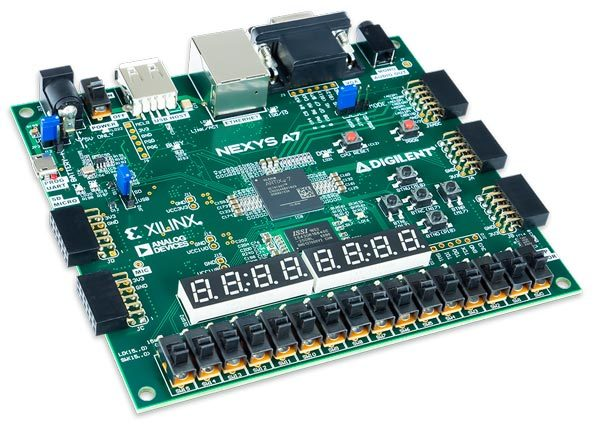
\includegraphics[width=10cm]{img/nexysa7.jpg}
\caption{\label{fig:nexys}Placa Nexys A7}
\end{center}
\end{figure}

Para el montaje de prototipo, se va a utilizar la placa proporcionada por el departamento: Nexys A7 de Digilent (figura \ref{fig:nexys}). Esta placa monta una FPGA de la familia Artix-7 modelo \emph{XC7A100T-1CSG324C} junto con múltiples opciones para conectividad, como son los puertos VGA, mini USB y Ethernet y para la entrada y salida de datos, como el micrófono, slot para microSD y sensor de temperatura y acelerómetro. Además incluye varios LED, que junto a los botones y conmutadores, permiten un cómodo manejo del conjunto de la placa. El conjunto de las prestaciones será más que suficiente para probar más adelante el funcionamiento de las características del prototipo.

De especial trascendencia para la puesta en marcha del conjunto, serán las bahías de pines que se ubican en ambos laterales de la Nexys, puesto que permiten conectar y leer los voltajes de entrada y salida que se van a emplear. La documentación proporcionada por Digilent \cite{Nexys} ha resultado muchas veces insuficiente, pero fundamental a la hora de poner en marcha el prototipo.

\section{Gestión entrada-salida}
Siguiendo el flujo de datos desde la etapa analógica, el siguiente paso consiste en introducir los mismos en la FPGA. Para ello, es imprescindible convertir el voltaje analógico en digital mediante el uso de un \emph{Conversor Analógico a Digital}, en lo sucesivo ADC. La Nexys A7 no incorpora ninguno integrado por lo que habrá que conectarlo externamente. Adelantando los acontecimientos, será necesario también un \emph{Conversor Digital a Analógico}, o DAC, para reconvertir a tensión analógica la salida de audio procesado. Por ello, se decide buscar ambos conversores conjuntamente, ya que se simplifica en gran medida la implemtación, ya que si son del mismo fabricante, suelen tener especificaciones de funcionamiento similares.

Exiten infinidad de este tipo de componentes en el mercado, todos ellos ideados para operar en diferentes condiciones de trabajo, en diferentes formatos y a un precio muy asequible. En el caso de las señales de audio, la mayor especificación que deben de cumplir es el compromiso de la tasa de muestreo $t_{s}$ (o más frecuentemente su inversa, la \emph{frecuencia de muestreo} $F_{s}$) para no corromper la señal entrante y preservar su calidad. Típicamente se utilizan algunos valores ya estandarizados por las grandes compañías de audio a lo largo del siglo XX:

\begin{itemize}
\item \textbf{$F_{s} = 8kHz$:} Utilizada especialmente para telefonía comercial pero no para componentes de audio de carácter musical.
\item \textbf{$F_{s} = 22050Hz$:} Frecuencia de muestreo típica de la radio que permite reproducir señales con componentes máximas de hasta 10kHz.
\item \textbf{$F_{s} = 32kHz$:} Se utiliza no tan frecuentemente en varios formatos de video digital, como el miniDV.
\item \textbf{$F_{s} = 44,1kHz$:} La más extendida en formatos como MP3, MPEG y CD por razones tanto históricas como prácticas. Puesto que un oído joven es capaz de percibir tonos de hasta 20kHz aproximadamente, esta tasa se estableció tras aplicar el criterio de Nyquist dejando un margen suficiente para compensar las etapas de filtrado posteriores.
\item \textbf{$F_{s} = 48kHz$:} También muy utilizada en televisión digital, DVD y audio profesional.
\item \textbf{$F_{s} = 96 o 192,4kHz$:} Pensada especialmente para audio de alta definición en formatos como HD-DVD y Blue-Ray Disc
\end{itemize}

Tras analizar las posibilidades, resulta evidente que para una aplicación de audio musical conviene establecer la frecuencia de muestro en 44,1 o 48 kHz de forma que conserve cierta similitud con los equipos comerciales y profesionales del mercado.

Así, aprovechando su reciente adquisición por parte del departamento, se va utilizar un componente que integre tanto ADC como DAC y que permita trabajar a estas velocidades: el \emph{Pmod i2s2} también de Digilent.

\subsection{Pmod i2s2}
Este componente trae, en definitiva todo lo necesario para este proyecto: junto a los ADC y DAC incorpora dos puertos para mini-jack estéreo hembra\footnote{Lo más extendido para audio, puesto que son los conectores que llevan móviles, auriculares. ordenadores, etc...} y una serie de pines dispuestos de tal forma que la conexión con la placa es inmediata. Se pueden observar estas características en la imagen \ref{fig:pmod}.

\begin{figure}[!ht]
\begin{center}
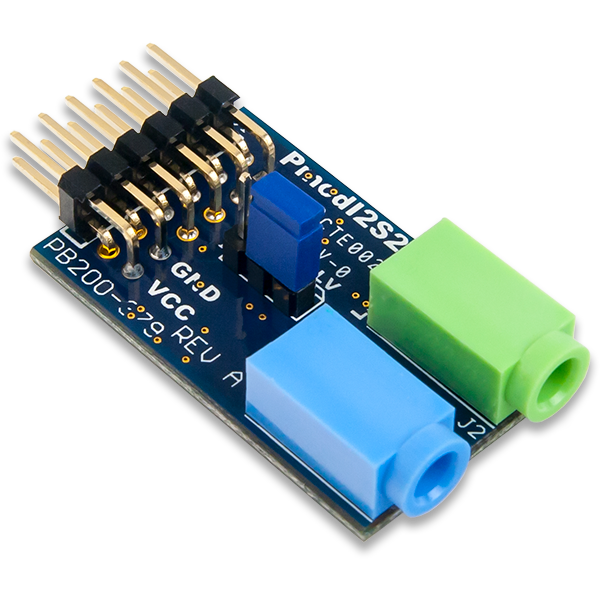
\includegraphics[width=6cm]{img/pmod.png}
\caption{\label{fig:pmod}Detalle del Pmod i2s2}
\end{center}
\end{figure}

Lógicamente, al ser ambos placa y \emph{plug-in} fabricados por Digilent, no hay ningún problema para conectarlos entre sí, basta con conectarlo a una de las bahías de pines que tiene la FPGA. Además, las conexiones de alimentación, Vcc y GND, se encuentran hechas de serie en la Nexys, por lo que no es necesario añadirlas en el fichero de conexiones o \emph{constraints}.

Tanto el modelo de ADC, \emph{Cirrus CS5345}, como el de DAC, \emph{Cirrus CS4344}
Hablar de las caracteristicas de ADC y DAC

\subsection{Consideraciones de implementación}
hablar de los relojes del vivado y sus problemas
archivo de constraints
\section{Controlador de datos}
h
\subsection{Bancos de memorias}
h
\subsection{Core FFT}
h
\section{Controlador global}
h
\subsection{Displays}
h 